\begin{figure}[h!]
  \begin{minipage}[c]{0.7\textwidth}
    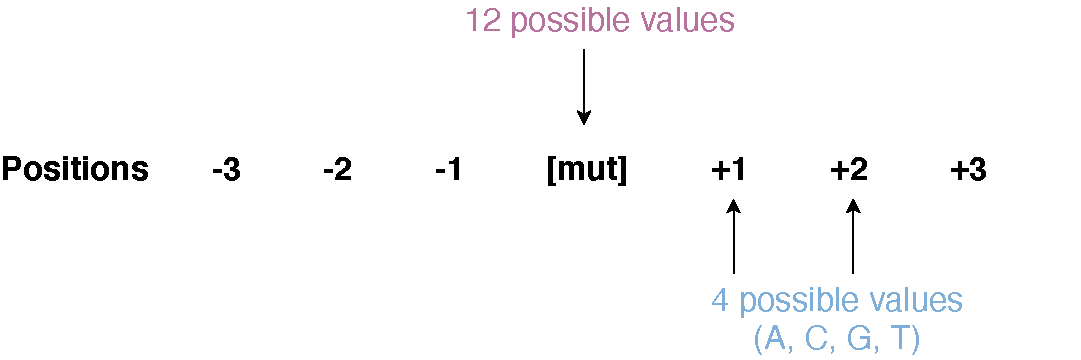
\includegraphics[width=\textwidth]{graphics/sce_counts_demo.pdf}
  \end{minipage}\hfill
  \begin{minipage}[c]{0.3\textwidth}
    \begin{equation}
    l = 12 \times 4^{k-1}
    \label{eq:sce_counts}
    \end{equation}
    where $l$ is the number of elements and $k$ is the k-mer size, so $k-1$ is the number of flanking bases involved
  \end{minipage}\hfill
  
  \vspace{0.5cm}
  \begin{minipage}[c]{\textwidth}
    \caption{
      \textbf{The number of elements increases extremely rapidly with increasing k-mer size, as per equation \ref{eq:sce_counts}.} This is because there are 12 possible mutations, and for each flanking position, there are 4 possible bases. 
    } \label{fig:sce_counts}
  \end{minipage}
\end{figure}
